
%
%  $Description: Author guidelines and sample document in LaTeX 2.09$
%
%  $Author: ienne $
%  $Date: 1995/09/15 15:20:59 $
%  $Revision: 1.4 $
%

\documentclass[12pt,twocolumn]{article}
\usepackage{latex8}
\usepackage{times}
\usepackage{graphicx}

%\documentstyle[times,art10,twocolumn,latex8]{article}

%-------------------------------------------------------------------------
% take the % away on next line to produce the final camera-ready version
\pagestyle{empty}

%-------------------------------------------------------------------------
\begin{document}

\title{Sketching Android Application GUIs}

\author{Will Hollingsworth, Steven Walker\\
College of William \& Mary\\ Department of Computer Science
}

\maketitle
\thispagestyle{empty}

\Section{Background and Motivation}
The development of a mobile application, in many cases, is a joint effort
between programmers and designers.  A designer will create a prototype of the
application GUI, which is then sent off to a programmer to implement.  However,
the designer typically has little to no experience with the actual implemenation
of such mock-ups, and this can result in a translation error between the
original mock-up and the final application.

IDEs like Android Studio include tools to design GUIs with a design that allows
users to drag and drop GUI elements onto a canvas and then export the design to
an XML file.  While this is a reasonalbe way to accomplish the tasks of UI
design, many designers perfer to draw their prototypes by hand, and such
electronic tools do little to replicate this type of workflow.

Therefore, it is desirable to create a tool that accepts as input a sketched
application prototype (or app screenshot), and then creates an application
skeleton whose GUI resembles the prototype.  Previous work has attempted to
mitigate this problem\cite{sketchit,mobidev}, but these either are not designed
with an Android environment in mind or are not suitable for deployment on a
laptop or desktop computer.

\SubSection{Previous Work: REMAUI}
REMAUI\cite{remaui}, developed by Tuan Nguyen and Cristoph Csallner, attempts to
solve this problem for input app screenshots.  Our project reimplements four of
the five major steps in the REAMUI approach.  We briefly outline it here.

The main idea behind the approach is to use the Tesseract Optical Character
Recognition (OCR) engine and Computer Vision (using the OpenCV library) to
identify the GUI elements in the input screenshot.  OCR algorithms are fairly
robust, and will identify text with little configureation, but they are not
perfect.  The false positive rate may be fairly high.  To account for this,
certain heurstics are used to remove likely false positives from consideration.
For example, the size of the word should not be zero and should contain actual
letters.

The computer vision step attempts to find bounding boxes for each major GUI
element and a heirarchy of those boxes.  It first runs the Canny edge detection
algorithm.  However, this isn't sufficient, as these edges would recognize
individual characters as GUI elements, which we certainly do not want.  To merge
such elements together, the image is dilated.  We then compute the bounding
boxes of the contours for each resulting visual element.  An initial view
hierarchy can be obtained from the hierarchy of contours.

REMAUI then merges the output of the previous two steps to update the hierarchy,
removing additional addtional false positive OCR results along the way.  In
order to create a more compact view hierarchy, we check for structural
repetitions in the current tree.  If, at any node, multiple child nodes have the
same number of children with roughly equivalent bounding boxes, we may classify
those subtrees as being in a list view.

The final hierarchy, along with all images and text, are then exported to an
Android project with XML resources and skeleton code.

\Section{Limiations of REMAUI}
REMAUI suffers from certain limitations that inhibit widespread use.  First and
foremost, it assumes that any non-text visual element is an image.  This means
that the resulting application cannot feature basic elements such as buttons and
spinners.  Moreover, the fact that the only elements available are text and
images implies that the resulting application will have no functionality.  It
will effectively consist of an Activity displaying the original screenshot.
Thus, while an application created by REMAUI could theoretically be deployed, it
would not be at all interactive.

The Canny edge detection algorithn requires finely tuned parameters that we were
unfortunately not able to approximate in our implemenation.  Notice in the
comparision in Figure \ref{fig:bbcompare} we are not able to pick up the
separator lines.  Although we did try various values for the \verb`lowThreshold`
and \verb`highThreshold` parameters, we were unable to detect them.  These
thresholds represent the intensity difference between pixels required to
classify it as an edge.  Once future avenue for finding the best
\verb`lowThreshold` might be identify the median intensity in the grayscaled
image on which the detection is done.  This should be relatively simple given
that there is only a single color channel.  Canny recommends using a value of 3
times the \verb`lowThreshold` for the \verb`highThreshold`.

The list detection method used by REMAUI looks at commonalites in children of
siblings in the view hierarchy.  But this requires that those siblings actually
be detected as vision blocks.  This is demonstrated by Figure
\ref{fig:bbcompare}.  Notice that REMAUI identifies a vision box for each
element in the message list.  Without the vision boxes containing the list
elements, it is impossible to remove the redundancies.

\begin{figure}[ht]
\centerline{
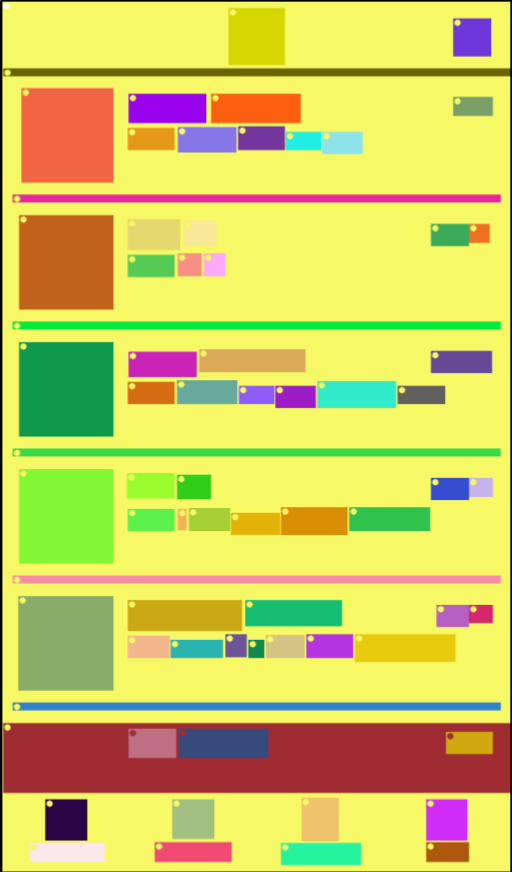
\includegraphics[width=0.5\columnwidth]{images/nguyenBoundingBoxes.png}
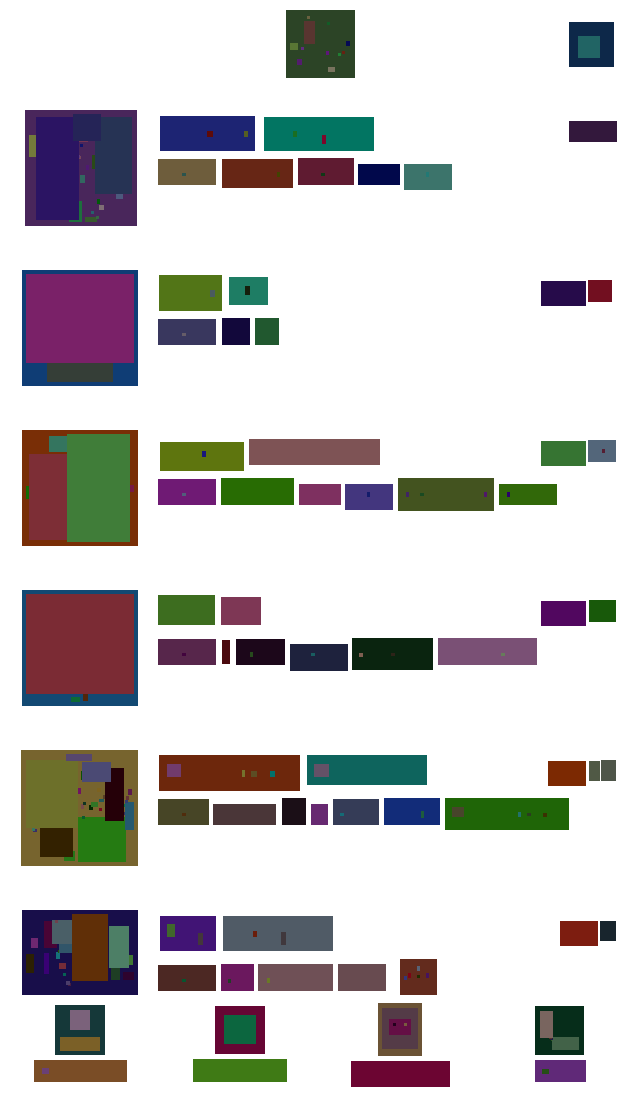
\includegraphics[width=0.5\columnwidth]{images/cv/contourBoundingBoxes.png}}
\caption{Left: The contour bounding boxes as detected by REMAUI  Right: The
contour bounding boxes as detected by our implementation.}
\label{fig:bbcompare}
\end{figure}

One of the heuristics REMAUI uses removes words that contain leaf vision boxes,
classifying them as false positives given that it contains a smaller visual
element.  One problem with this is that, since the contours of letters bleed
together when dilating them, contours might be picked up for the letter counters
(the inside of a letter such as ``P'' or ``O'').  Since we would detect a
contour for the counter and the full letter, this would throw off the heuristic.

Another, less serious limitation is that the implementation is closed source, and
can only be used via a web-based front end.  That is, it cannot be run offline.

\Section{Our Implementation}
\begin{figure*}[ht]
\centerline{
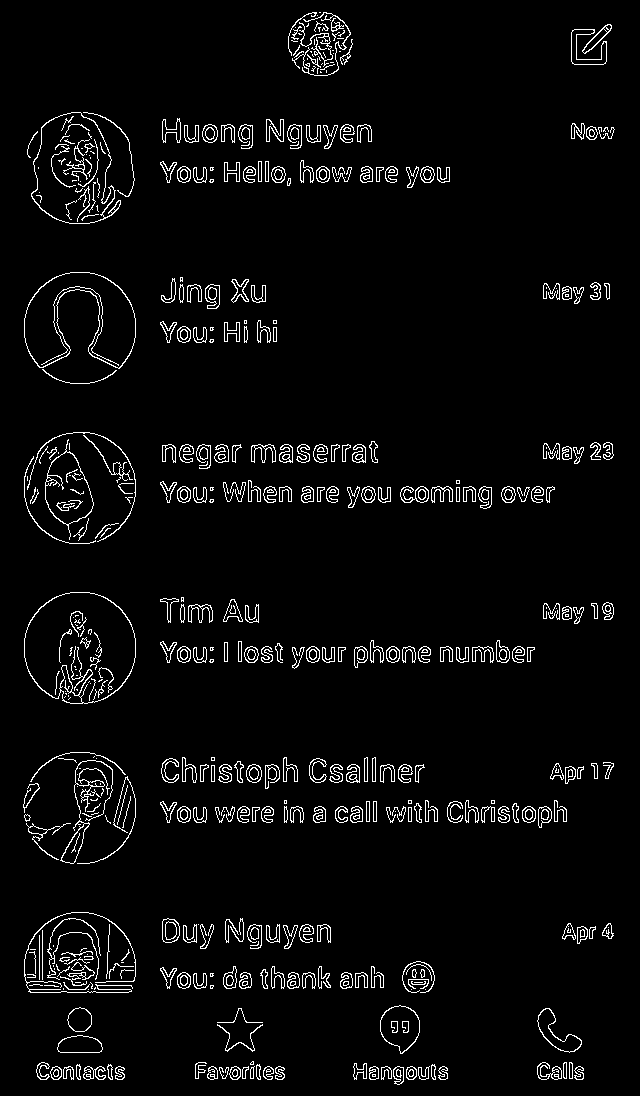
\includegraphics[width=0.5\columnwidth]{images/cv/canny.png}
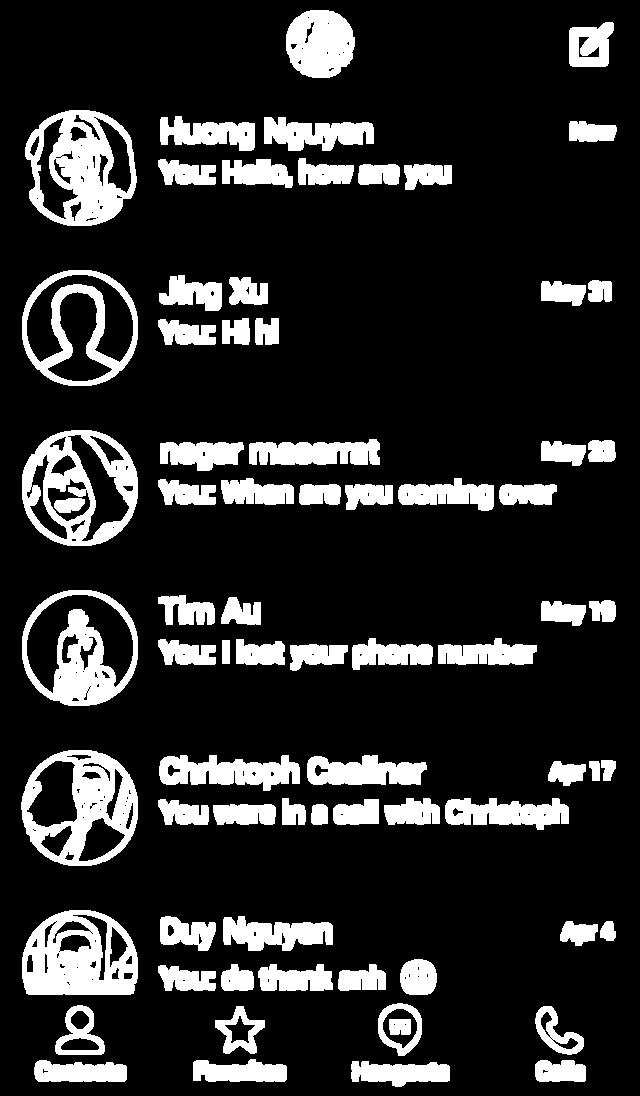
\includegraphics[width=0.5\columnwidth]{images/cv/dilate.png}
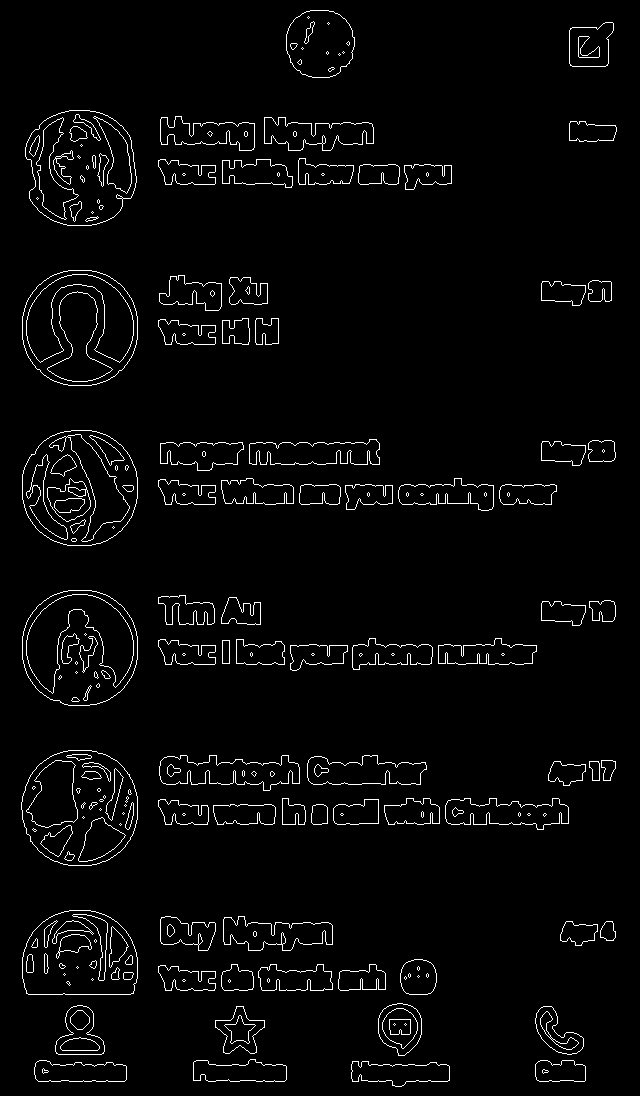
\includegraphics[width=0.5\columnwidth]{images/cv/contours.png}
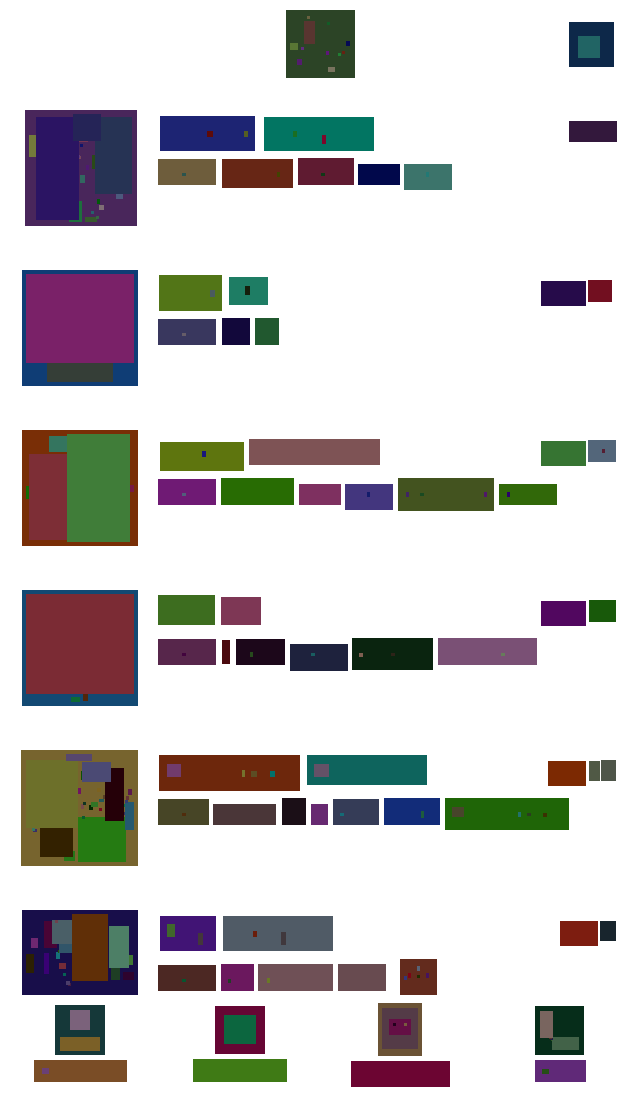
\includegraphics[width=0.5\columnwidth]{images/cv/contourBoundingBoxes.png}}
\caption{The results of the Canny edge detection, edge dilation, the contours of
the resulting shapes, and the bounding boxes of the contours.}
\label{fig:cvresults}
\end{figure*}

\begin{figure*}[ht]
\centerline{
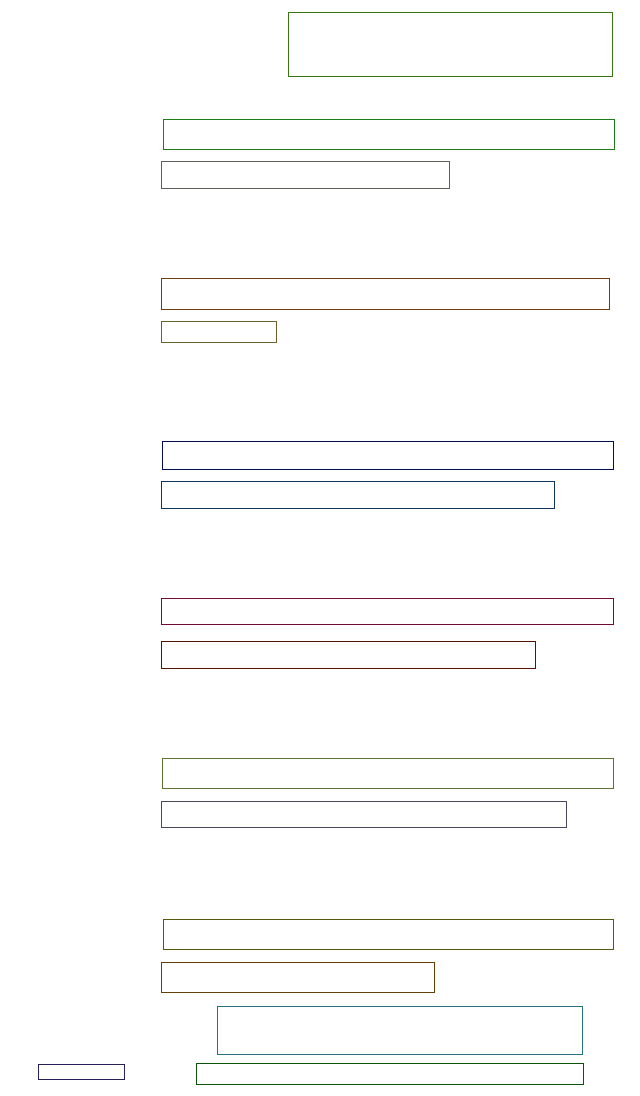
\includegraphics[width=0.5\columnwidth]{images/ocr/lineBoundingBoxes.png}
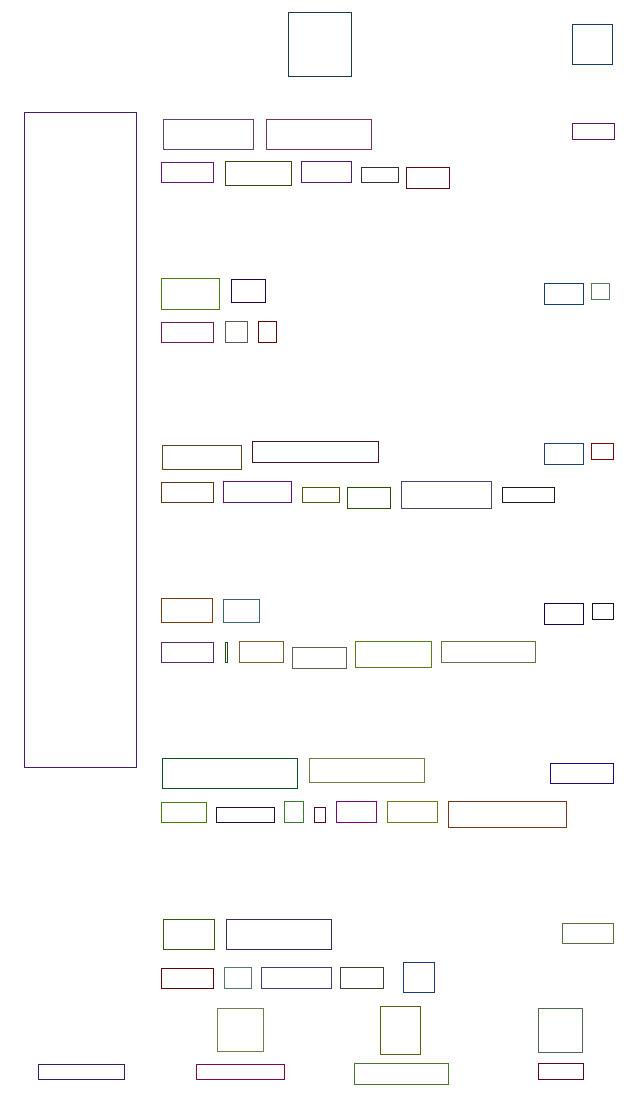
\includegraphics[width=0.5\columnwidth]{images/ocr/wordBoundingBoxes.png}
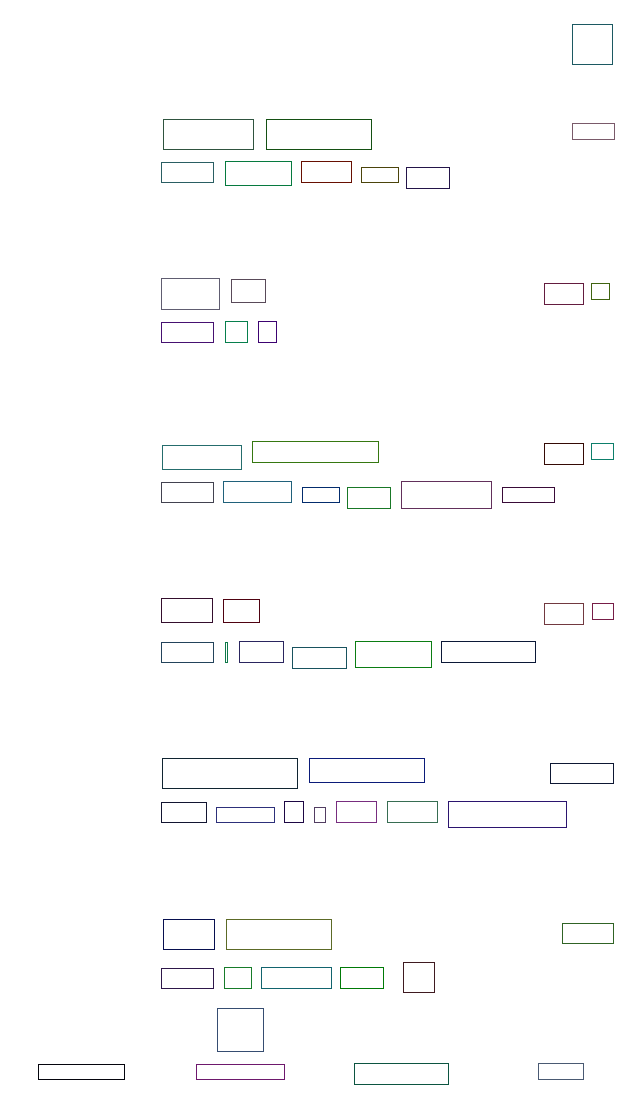
\includegraphics[width=0.5\columnwidth]{images/ocr/filteredBoundingBoxes.png}
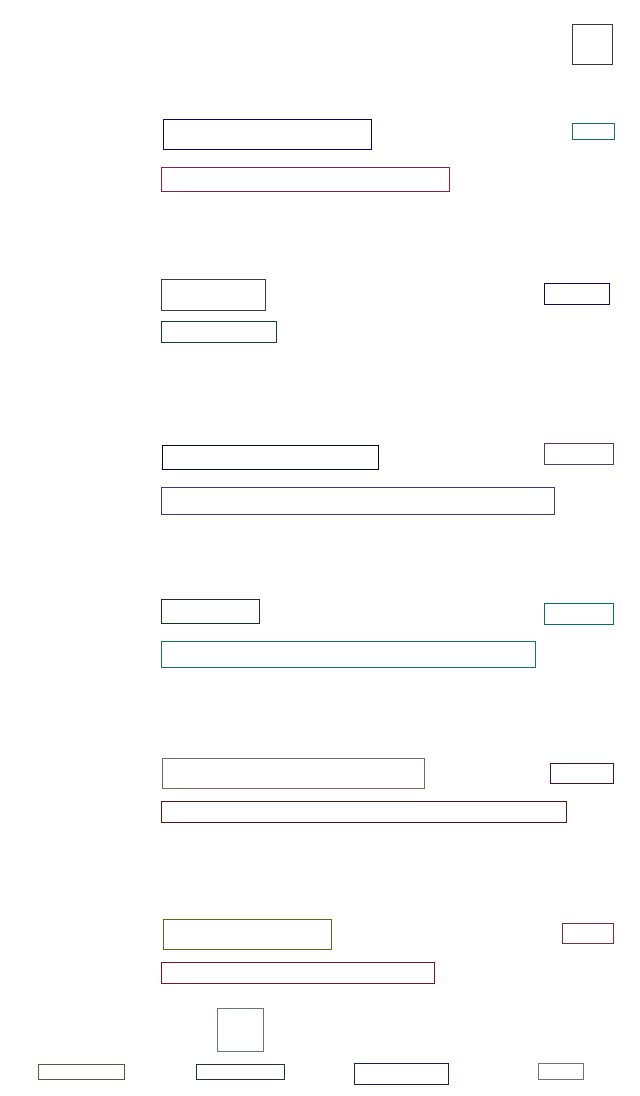
\includegraphics[width=0.5\columnwidth]{images/ocr/blockBoundingBoxes.png}}
\caption{From left to right: The bounding boxes of the lines detected by OCR,
the bounding boxes of the words, the bounding boxes of the words after filtering
false positives, and the bounding boxes of the final text blocks.}
\label{fig:ocrresults}
\end{figure*}

We reimplemented the first four steps of the REMAUI approach in our tool.
Rather than generate a complete Android project, we create (for now) only a
\verb`layout.xml` file.  Our results from OpenCV are displayed in Figure
\ref{fig:cvresults} and results from OCR are displayed in Figure
\ref{fig:ocrresults}.

Note that the large amount of noise in the vision boxes detected by OpenCV is
accounted for by, for any image view, removing its children if they are all
image views as well.

\Section{Future Work}
To solve the problems of the REMAUI approach, we propose an extended workflow.

After computing the application's view hierarchy, we propose exporting images of
the individual GUI element, the location of that element on the screen, and any
text associated with that element.  Using a database of existing applications
with annotated GUI elements, we can construct a corpus of GUI elements that
capture their salient features.

This corpus would then be fed into a recurrent neural network along with the
visual elements detected by the REMAUI approach.  The RNN would be able to
classify the type of each element in the input sketch or screenshot using the
GUI element corpus.  Using these classifications, we can update the view
hierarchy of the application to generate.

Finally, the updated hierarchy can be compared to the hierarchies of the
applications in the database using a code search method such as CLAN\cite{clan}.
The reasoning behind this step is that an application with a similar heirarchy
of GUI elements may be implementing similar functionality.  This would allow us
to fill in basic functionality such as transitions between activities in the
application.
%-------------------------------------------------------------------------
\nocite{*}
\bibliographystyle{latex8}
\bibliography{report}

\end{document}

